\chapter{Usage of Annotations -- Fuzzy ILP Document Classification}

\graphicspath{{../img/ch80/}}


%%%%%%%%%%%%%%%%%%%%%%%%%%%%%%%%%%%%%%%%%%%%%%%%%%%%%%%%%%%%%%%%%%%%%%%%%%%%%%%%%%%%%%%%%%%%%%%%%
\section{Introduction}
%%%%%%%%%%%%%%%%%%%%%%%%%%%%%%%%%%%%%%%%%%%%%%%%%%%%%%%%%%%%%%%%%%%%%%%%%%%%%%%%%%%%%%%%%%%%%%%%%

The vast amount of information on the web increases the need of automated processing. Machine processing and machine understanding of textual information is especially difficult. In this chapter we study the problem of classification of textual web reports. We are specifically focused on the situations in which structured information extracted from the reports is used for such classification. We present an experimental classification system based on usage of third party linguistic analyzers, our previous work on web information extraction and fuzzy inductive logic programming (fuzzy ILP).

\begin{figure}
\centerline{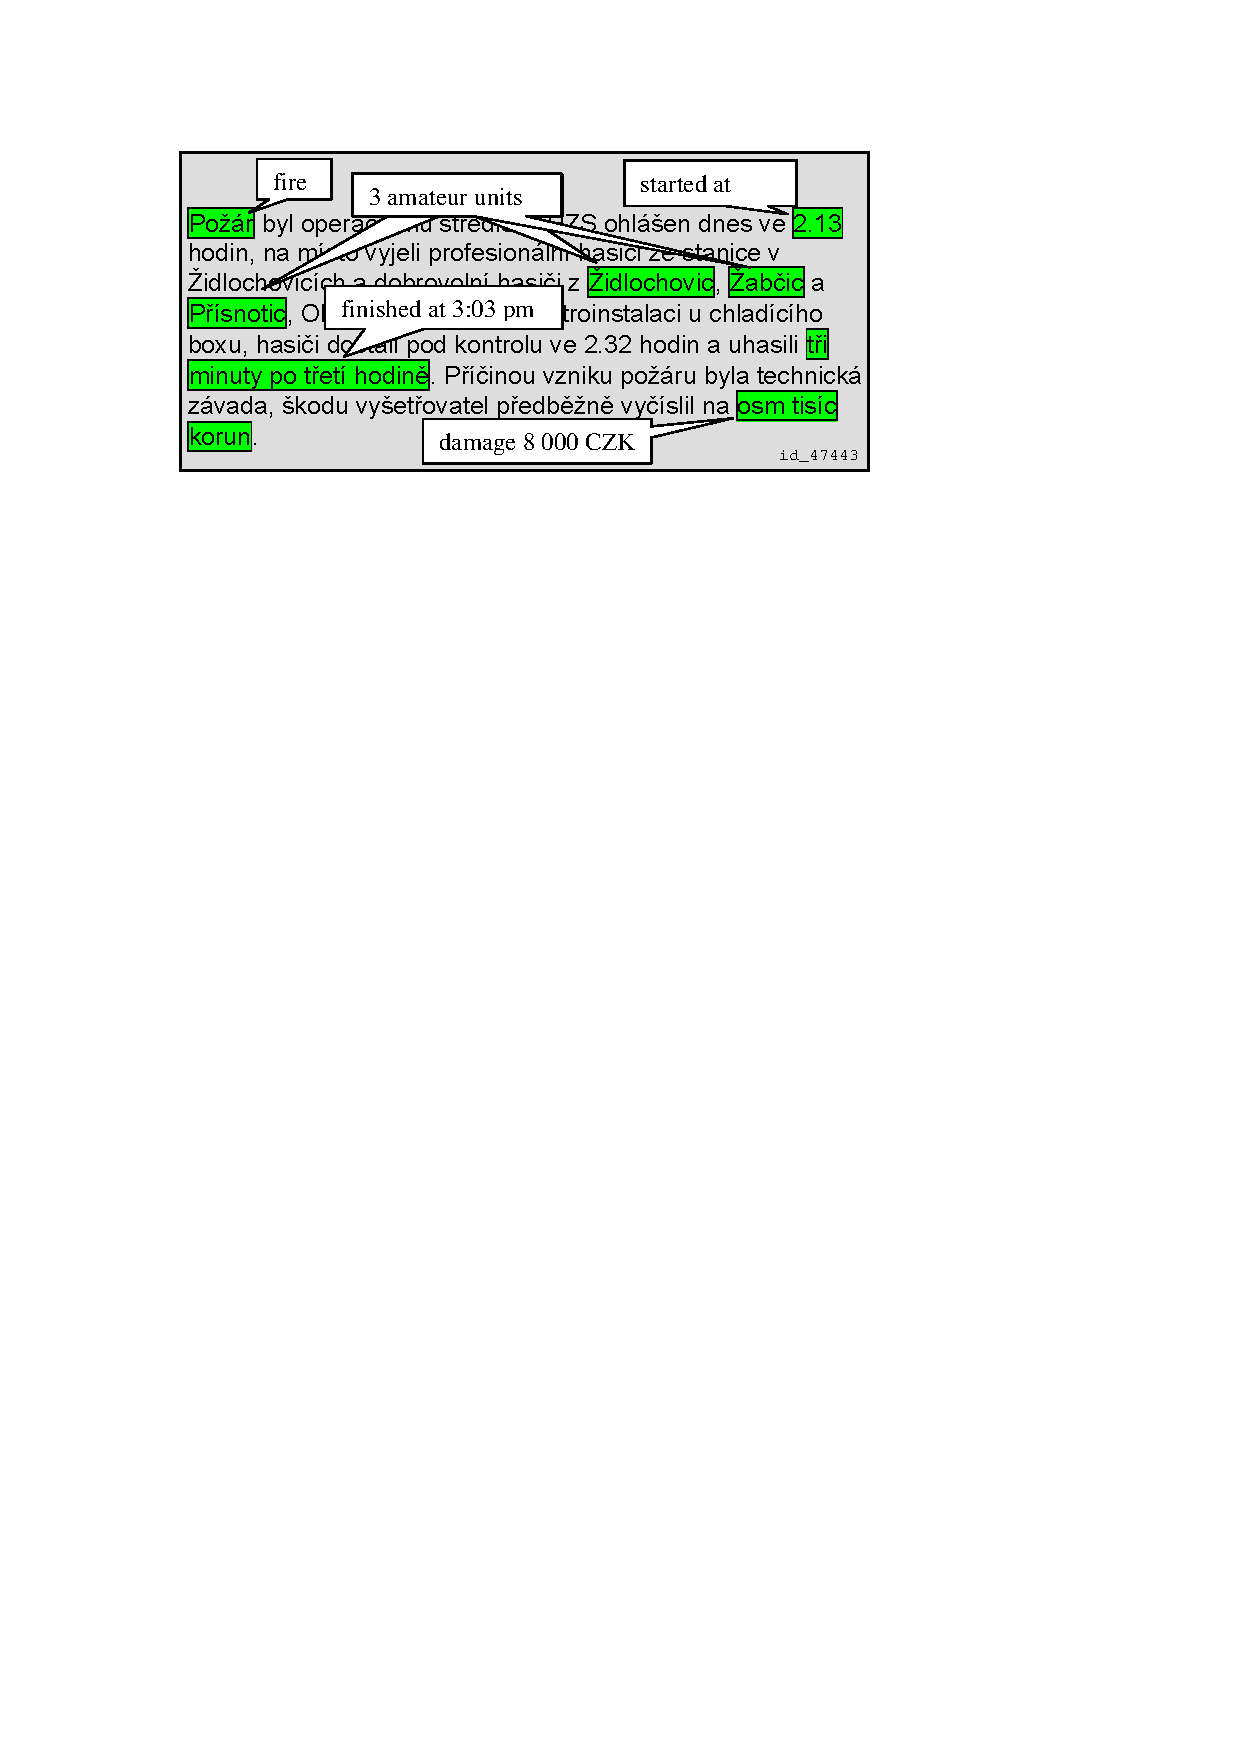
\includegraphics[width=0.7\hsize]{message}}
\caption{Example of analyzed web report.}
\label{img:message}
\end{figure}


The chapter is based on a case study of seriousness classification of accident reports. Fig.~\ref{img:message} presents an example of an accident report from a message on the web. We would like to have a tool that is able to classify the accident's degree of seriousness in such a message.

Our solution is based on information extraction (see emphasized pieces of information that could be extracted from a report in Fig.~\ref{img:message}) and on a fuzzy-based machine learning procedure that provides rules for classification of the reports.

Our experiments deal with texts in the Czech language but our method is general and it can be used with any structured linguistic representation. In this chapter we do not provide many details about the information extraction part of the solution. We concentrate on the classification part and present a detailed study of the fuzzy ILP classification method (so-called `Fuzzy ILP Classifier'). 

In our application we are facing the challenge of induction and/or mining on several occasions. First we need an inductive procedure when extracting attributes of an accident from text. Second (the subject of this chapter) we need an inductive procedure when trying to explain an accident's degree of seriousness by its attributes. ILP is used as the inductive procedure in both of these places.
\begin{itemize}
	\item During the information extraction phase, we exploit the fact that ILP can work directly with multirelational data, e.g., deep syntactic (tectogrammatical) trees built from sentences of the processed text.
	\item During the classification phase, we are experimentally using the Fuzzy ILP Classifier because it performs quite well on our dataset (see Section~\ref{sec:ch80_eval}) and it is naturally capable of handling fuzzy data, which occurs when the information extraction engine returns confidence probability values along with extracted data. But the description does not go so far and only the approach is fuzzy in the present demonstration.
\end{itemize}

The main \emph{contributions} presented in this chapter are \emph{formal models}, prototype \emph{implementation} and experimental \emph{evaluation} of the Fuzzy ILP Classifier.
\medskip

The chapter is organized as follows: In Section~\ref{sec:related} we introduce some closely related works. Design of the experimental system is presented in Section~\ref{sec:system}, including a short description of the information extraction method and linguistic analyzers. Section~\ref{sec:ch80_case} provides details about our case study, which is later used in examples. Formal models of the system (including ILP, fuzzy ILP and several translations of a fuzzy ILP task to classical ILP) are presented in Section~\ref{sec:ILP}, followed by a description of implementation of the models in the system. In Section~\ref{sec:results} we present the main results of the work, and then we evaluate and compare the methods with other well-known classifiers. Section~\ref{sec:conclusion} concludes the paper.

 


%%%%%%%%%%%%%%%%%%%%%%%%%%%%%%%%%%%%%%%%%%%%%%%%%%%%%%%%%%%%%%%%%%%%%%%%%%%%%%%%%%%%%%%%%%%%%%%%%
\section{Related Work} \label{sec:related}
%%%%%%%%%%%%%%%%%%%%%%%%%%%%%%%%%%%%%%%%%%%%%%%%%%%%%%%%%%%%%%%%%%%%%%%%%%%%%%%%%%%%%%%%%%%%%%%%%

There are plenty of systems dealing with text mining and text classification. In \citep{dedek:ReYaLiOntoText08} the authors use ontology modeling to enhance text identification. The authors of \citep{dedek:CAP} use preprocessed data from National Automotive Sampling System and test various soft computing methods to model severity of injuries (some hybrid methods showed best performance). Methods of Information Retrieval (IR) are numerous, with extraction mainly based on key word search and similarities. The Connection of IR and text mining techniques with web information retrieval can be found in the chapter ``Opinion Mining�� in the book of Bing Liu \citep{dedek:WebDataMining}. 

The Fuzzy ILP Classifier can be seen as an ordinary classifier for data with the monotonicity constraint (the target class attribute has to be monotonizable -- a natural ordering has to exist for the target class attribute). There are several other approaches addressing the classification problems with the monotonicity constraint.

The CART-like algorithm for decision tree construction does not guarantee a resulting monotone tree even on a monotone dataset. The algorithm can be modified \citep{dedek:mon_trees} to provide a monotone tree on the dataset by adding the corner elements of a node with an appropriate class label to the existing data whenever necessary.

An interesting approach is presented in \citep{dedek:mon_transf}: first, the dataset is ``corrected'' to be monotone (a minimal number of target class labels is changed to get a monotone dataset), then a learning algorithm (linear programming boosting in the cited paper) is applied.

Several other approaches to monotone classification have been presented, including instance based learning \citep{dedek:ibl} and rough sets \citep{dedek:rough_sets}.





%%%%%%%%%%%%%%%%%%%%%%%%%%%%%%%%%%%%%%%%%%%%%%%%%%%%%%%%%%%%%%%%%%%%%%%%%%%%%%%%%%%%%%%%%%%%%%%%%
\section{Design of the system} \label{sec:system}
%%%%%%%%%%%%%%%%%%%%%%%%%%%%%%%%%%%%%%%%%%%%%%%%%%%%%%%%%%%%%%%%%%%%%%%%%%%%%%%%%%%%%%%%%%%%%%%%%
\begin{figure}
\centerline{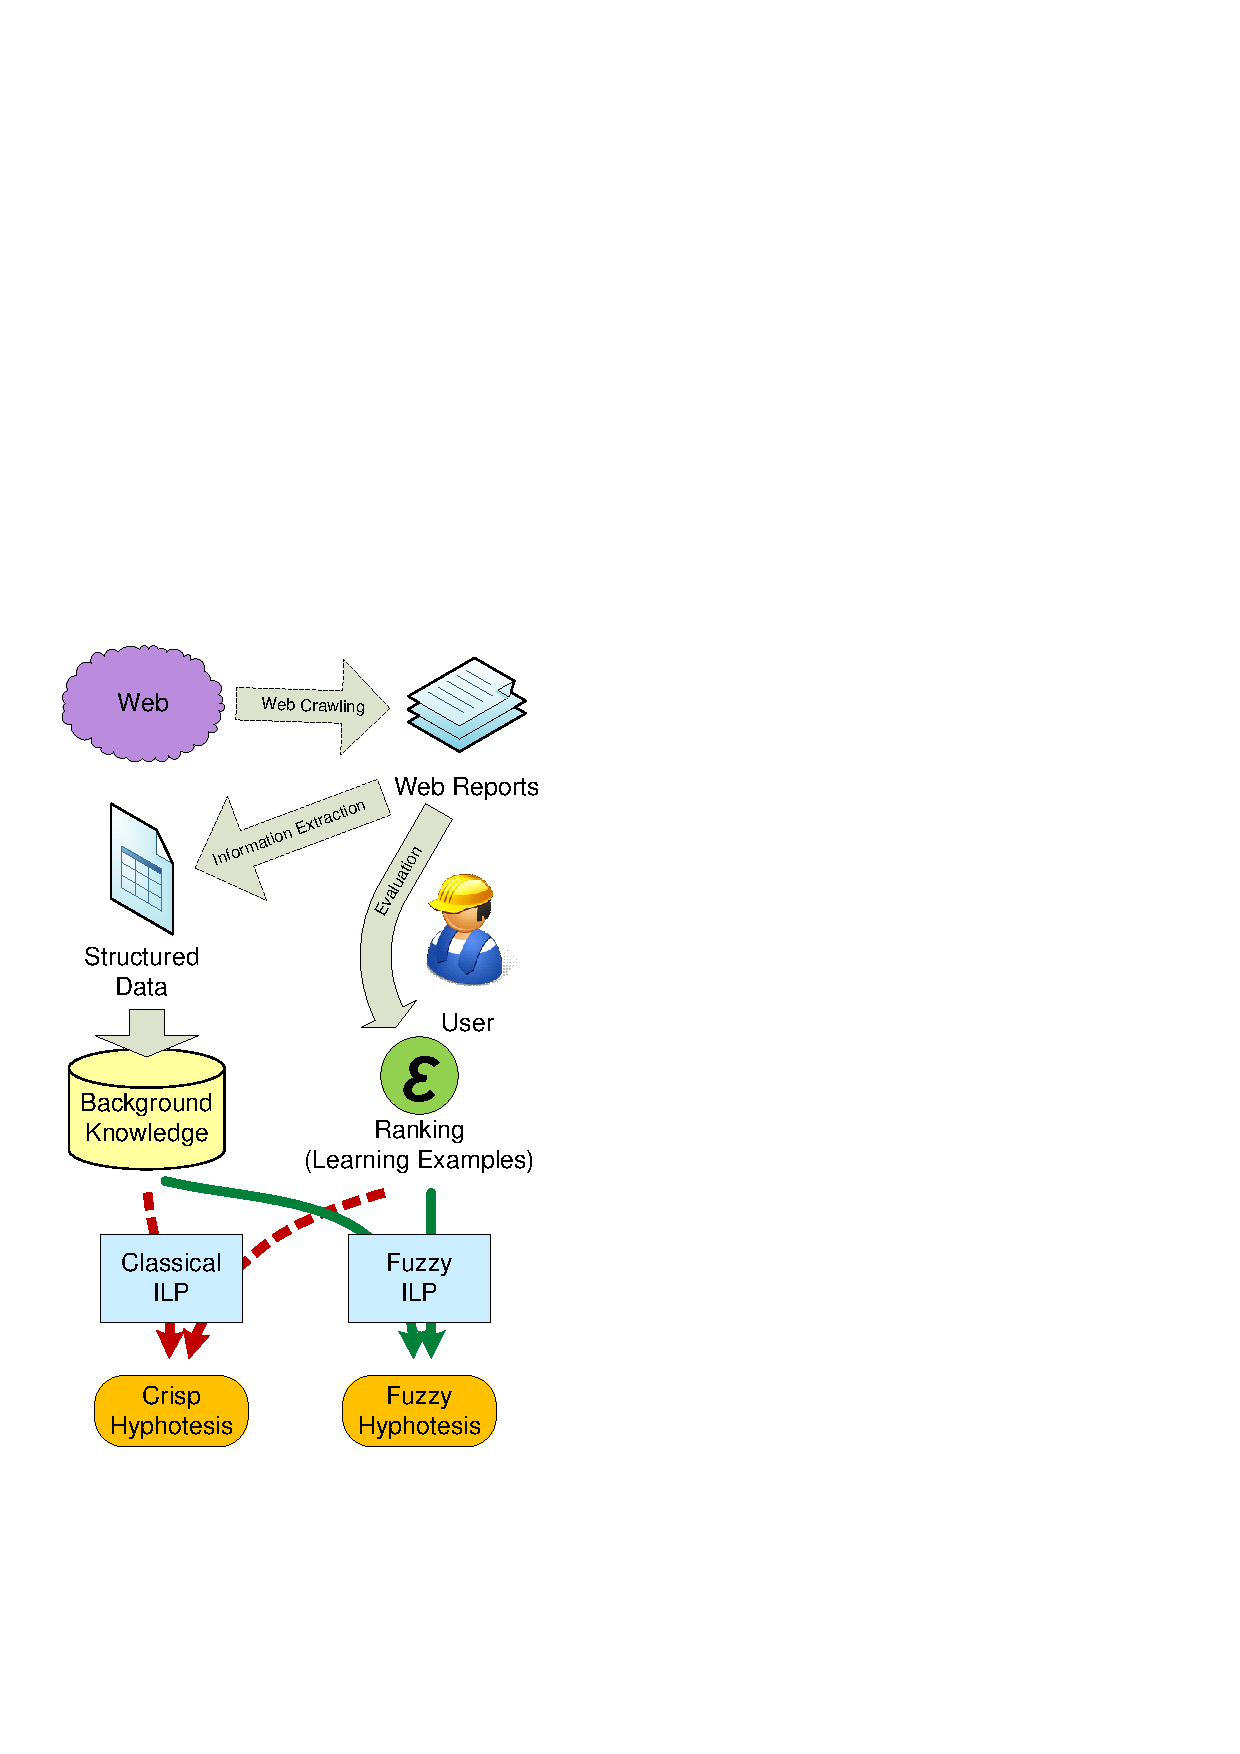
\includegraphics[width=0.4\hsize]{schema}}
\caption{Schema of our system.}
\label{img:schema}
\end{figure}

%\begin{floatingfigure}[r]{.45\hsize}
%\centerline{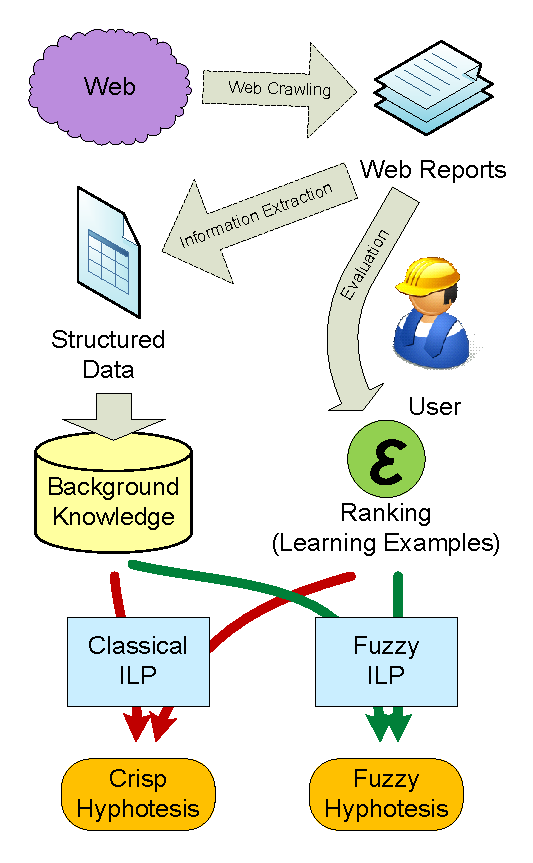
\includegraphics[width=\hsize]{img/schema}}
%\caption{Schema of the whole system.}
%\label{img:schema}
%\end{floatingfigure}

A general schema of our experimental system is shown in Fig.~\ref{img:schema}. We use our previously developed web information extraction tools based on third party linguistic analyzers (the upper two dashed arrows; this is not a subject of this chapter). We extract some structured information from the web and the extracted information is then translated to an ILP knowledge base and, along with a user rating, it is used for the classification (we assume that a small amount of learning data is annotated by a human user). The classification is based on ILP and it could be \emph{fuzzy} or \emph{crisp}. Crisp denotes a straightforward application of ILP and fuzzy stands for the fuzzy method (subject of the paper), see in the next sections.



%%%%%%%%%%%%%%%%%%%%%%%%%%%%%%%%%%%%%%%%%%%%%%%%%%%%%%%%%%%%%%%%%%%%%%%%%%%%%%%%%%%%%%%%%%%%%%%%%
\subsection{Linguistic Analysis}
%%%%%%%%%%%%%%%%%%%%%%%%%%%%%%%%%%%%%%%%%%%%%%%%%%%%%%%%%%%%%%%%%%%%%%%%%%%%%%%%%%%%%%%%%%%%%%%%%

In this section we will briefly describe the linguistic tools that
we have used to produce linguistic annotations of texts. 
These tools are being developed in the Institute of Formal
and Applied Linguistics in Prague, Czech Republic. They
are publicly available -- they have been published on a CDROM
under the title PDT 2.0 (\cite{dedek:PDT20_CD} -- the first five tools) and in
(\cite{dedek:KlTransformationBasedTectogrammatical2006} -- Tectogrammatical analysis). These tools are used as a
processing chain. At the end of the chain they produce
tectogrammatical dependency trees \citep{dedek:MiBeAnnotationtectogrammatical2006} built up from the text.


\begin{description}
 
	\item[Tool 1.] Segmentation and tokenization consists of dividing the input text into words and punctuation (tokenization) and dividing a sequence of tokens into sentences (segmentation).

	\item[Tool 2.] Morphological analysis assigns all possible lemmas
and morphological tags to particular word forms (word
occurrences) in the text.

	\item[Tool 3.] Morphological tagging consists in selecting a single
pair lemma-tag from all possible alternatives assigned
by the morphological analyzer.

	\item[Tool 4.] Collins' parser -- Czech adaptation. 
Unlike the usual approaches to the description of
English syntax, the Czech syntactic descriptions are
dependency-based, which means that every edge of
a syntactic tree captures the relation of dependency
between a governor and its dependent node. Collins'
parser gives the most probable parse of a given input
sentence.

	\item[Tool 5.] Analytical function assignment assigns a description
(analytical function, in linguistic sense) to every edge
in the syntactic (dependency) tree.

	\item[Tool 6.] Tectogrammatical analysis produces linguistic annotation
at the tectogrammatical level, sometimes called
``layer of deep syntax''. An example of a tectogrammatical tree can be seen in
Fig.~\ref{img:ch80_tree}. Annotation of a sentence at this layer
is closer to the meaning of the sentence than its syntactic
annotation; thus, information captured at the tectogrammatical
layer is crucial for machine understanding
of natural language \citep{dedek:KlTransformationBasedTectogrammatical2006}.
\end{description}


%%%%%%%%%%%%%%%%%%%%%%%%%%%%%%%%%%%%%%%%%%%%%%%%%%%%%%%%%%%%%%%%%%%%%%%%%%%%%%%%%%%%%%%%%%%%%%%%%
\subsection{Web Information Extraction}
%%%%%%%%%%%%%%%%%%%%%%%%%%%%%%%%%%%%%%%%%%%%%%%%%%%%%%%%%%%%%%%%%%%%%%%%%%%%%%%%%%%%%%%%%%%%%%%%%

After the content of a web resource is analyzed by the above-mentioned linguistic tools, the output linguistic data is obtained in the form of tectogrammatical trees. To achieve our objectives we have to extract information from this representation. 
Here we refer to our previous work %\citep{dedek:DeVoComputingaggregations2008,dedek:DeVoLinguisticextraction2008,dedek:DeEcExperimentswith2008}.
\citep{dedek:DeVoComputingaggregations2008,dedek:DeEcExperimentswith2008}.
 A long path of tools, starting with web crawling and resulting in the extracted structured information, has been developed in our previous works. 
In Fig.~\ref{img:ch80_tree}, nodes of the tectogrammatical tree are decorated. A piece of information about the damage of 8000 CZK can be found there (the three nodes on the right). We have used ILP to learn rules that are able to detect these nodes. 
%In this paper we will concentrate on the usage of such extracted information to be able to classify content. 
The extraction process requires human assistance when annotating the training data.

Note that our method is general and is not limited to Czech. It can be used with any structured linguistic representation. 


\begin{figure}
\centerline{\framebox{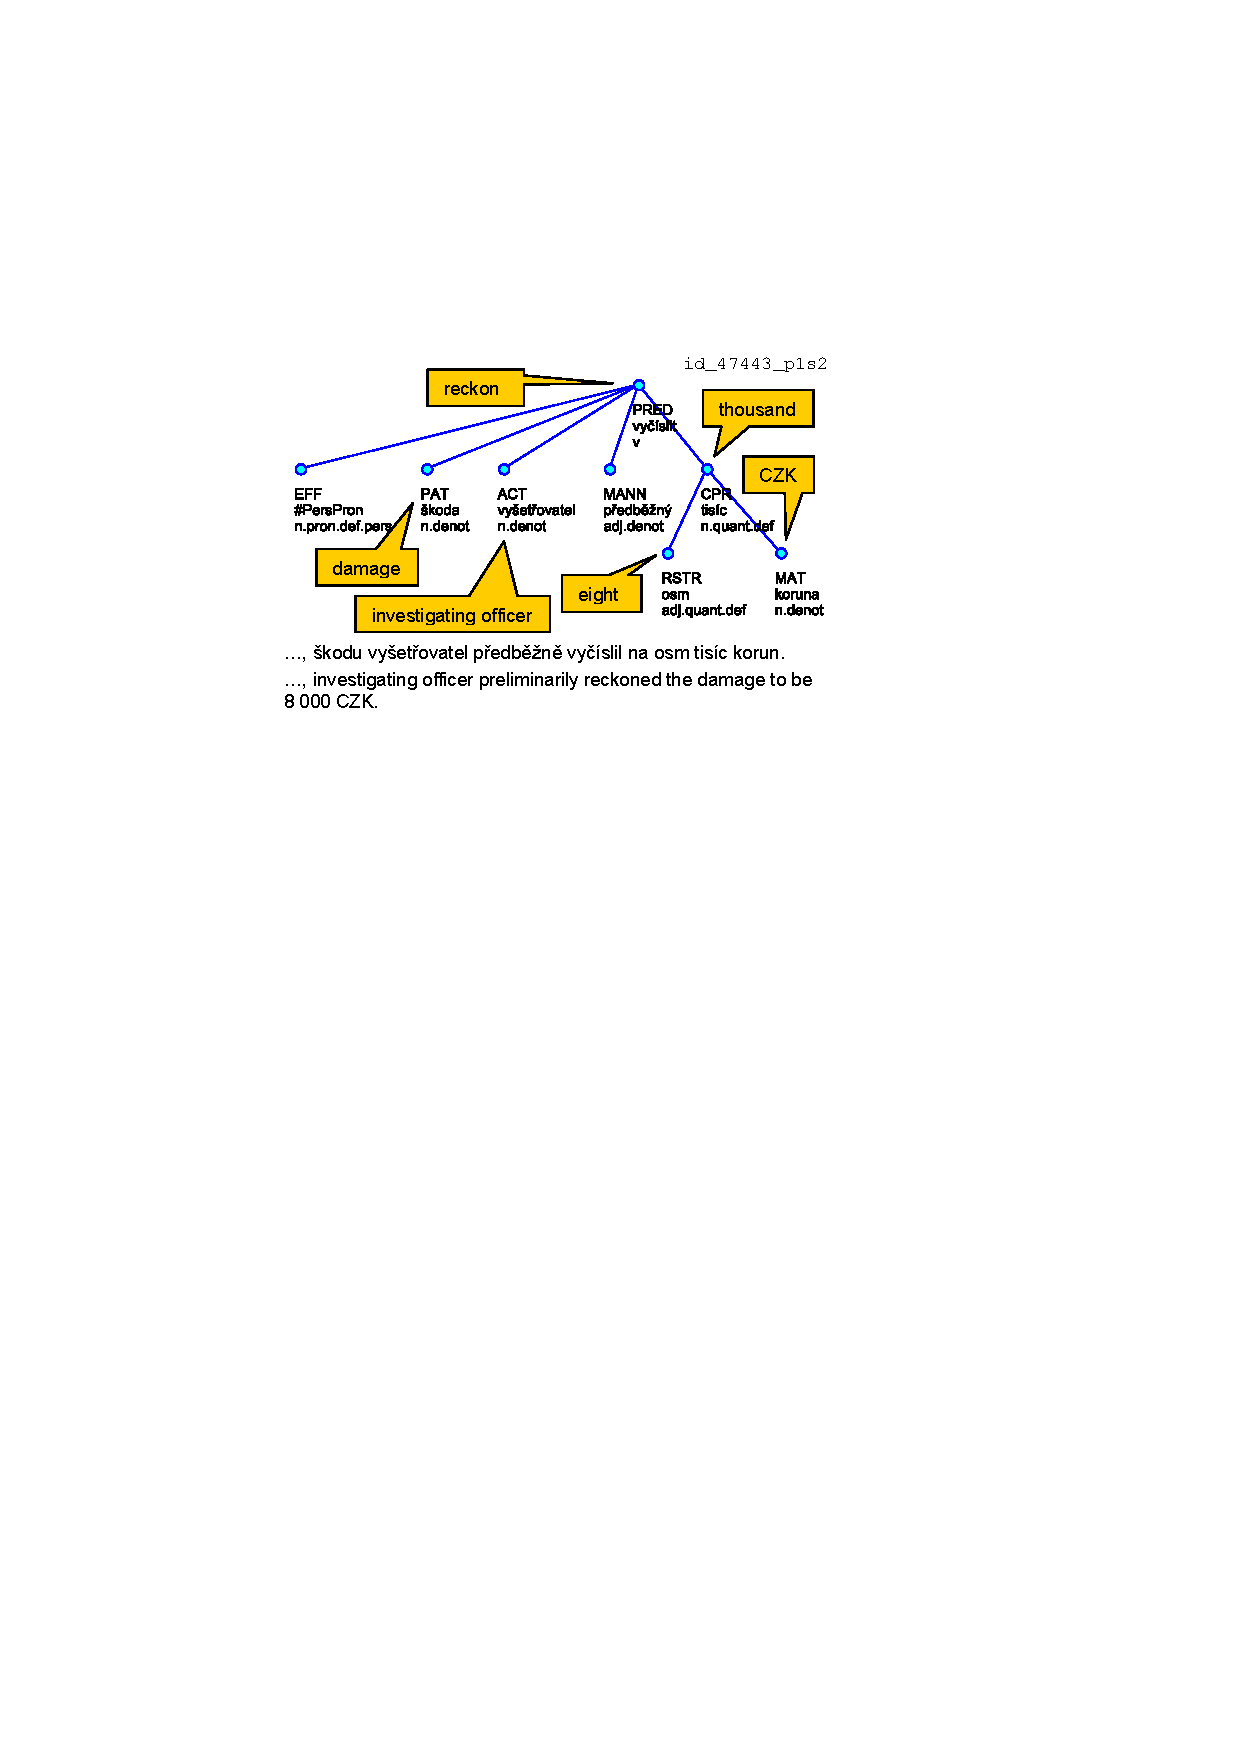
\includegraphics[width=0.7\hsize]{tree}}}
\caption{Example of a linguistic tree of one analyzed sentence.}
\label{img:ch80_tree} \label{img:damage_tree}
\end{figure}














%%%%%%%%%%%%%%%%%%%%%%%%%%%%%%%%%%%%%%%%%%%%%%%%%%%%%%%%%%%%%%%%%%%%%%%%%%%%%%%%%%%%%%%%%%%%%%%%%
\section{The case study -- accident seriousness classification} \label{sec:ch80_case}
%%%%%%%%%%%%%%%%%%%%%%%%%%%%%%%%%%%%%%%%%%%%%%%%%%%%%%%%%%%%%%%%%%%%%%%%%%%%%%%%%%%%%%%%%%%%%%%%%



The main experiment presented in this chapter leads to the seriousness classification of an accident presented in a web report. %Our long term goal is extraction of semantic information from web reports. 
%which is one of possible utilizations of the extracted information. 
We use online fire department reports from several regions of the Czech Republic. These reports are written in Czech and can be accessed through the web of the General Directorate of the Fire and Rescue Service of the Czech Republic\footnote{\url{http://www.hzscr.cz}}. 
%These reports are rich in information, e.g. where and when an traffic accident occurred, which units helped, how much time it took them to show up on the place of accident, how many people were injured, killed etc.

For our experiment we have selected a collection of 50 web reports. We have identified several features presented in these reports and manually extracted the corresponding values. This will be described in more detail in Section \ref{sec:features}. To each report we have also assigned a value of overall ranking of seriousness of the presented accident, which is the target of the classification. The whole dataset can be downloaded from our Fuzzy ILP classifier's web page\footnote{\url{http://www.ksi.mff.cuni.cz/~dedek/fuzzyILP/}}.

In this experiment we have not used any information extracted by our automated information extraction tools. Instead, we concentrate on~the classification; the actual source of the information is not so important. The integration step still lies ahead.

%There are two objectives to do. Fist is the web information extraction, a long path starting with web crawling and resulting with the extracted structured information. Second is the seriousness classification, which utilizes the extracted information. We have made much work on the first (see e.g. %\citep{biblio:DeVoLinguisticextraction2008,biblio:DeVoComputingaggregations2008, biblio:DeEcExperimentswith2008}), in this paper we will concentrate on the second.
%\citep{biblio:DeEcExperimentswith2008}), in this paper we will concentrate on the second.




\begin{table}
\centering
\begin{tabular}{|r||c|c|c|}
\hline
attribute name & distinct values & missing values & monotonic\\
\hline
\hline
size (of file) & 49 & 0 & yes\\
\hline
type (of accident) & 3 & 0 & no\\
\hline
damage & 18 & 30 & yes\\
\hline
dur\_minutes & 30 & 17 & yes\\
\hline
fatalities & 4 & 0 & yes\\
\hline
injuries & 5 & 0 & yes\\
\hline
cars & 5 & 0 & yes\\
\hline
amateur\_units & 7 & 1 & yes\\
\hline
profesional\_units & 6 & 1 & yes\\
\hline
pipes & 7 & 8 & yes\\
\hline
lather & 3 & 2 & yes\\
\hline
aqualung & 3 & 3 & yes\\
\hline
fan & 3 & 2 & yes\\
\hline
ranking & 14 & 0 & yes\\
\hline
\end{tabular}

\caption{Accident attributes.}
\label{img:attributes_description}
\end{table}


%%%%%%%%%%%%%%%%%%%%%%%%%%%%%%%%%%%%%%%%%%%%%%%%%%%%%%%%%%%%%%%%%%%%%%%%%%%%%%%%%%%%%%%%%%%%%%%%%
\subsection{Features of accidents} \label{sec:features}
%%%%%%%%%%%%%%%%%%%%%%%%%%%%%%%%%%%%%%%%%%%%%%%%%%%%%%%%%%%%%%%%%%%%%%%%%%%%%%%%%%%%%%%%%%%%%%%%%


Table~\ref{img:attributes_description} summarizes all features (or attributes) that we have obtained from accident reports. Except for the attribute \verb+type+ (type of an accident -- \verb+fire+, \verb+car_accident+ and \verb+other+), all the attributes are numerical and therefore \emph{monotonizable} (see the next sections). There are cases in which the value of an attribute is unknown. We have decided to make evidence of this and keep the values \verb+unknown+ in the knowledge base. A brief explanation of each attribute follows.
\begin{itemize}
	\item \verb+size+ is length of text of a particular report.
	\item \verb+damage+ is an amount (in CZK -- Czech Crowns) of summarized damage arisen during a reported accident.
	\item \verb+dur_minutes+ is time taken to handle an accident.
	\item \verb+fatalities+ and \verb+injuries+ are numbers of deaths and wound people sustained in an accident.
	\item \verb+cars+ is the number of vehicles damaged during an accident (mostly during car accidents).
	\item \verb+professional_units+ and \verb+amateur_units+ are numbers of fireman and volunteer units sent for a particular accident.
	\item \verb+pipes+ is a number of used fire hoses.
	\item \verb+lather+, \verb+aqualung+ and \verb+fan+ (ventilator) indicates whether these devices were used.
\end{itemize}

A majority of accidents are of the type \verb+fire+ (52\%)
and \verb+car_accident+ (30\%),
the rest (type \verb+other+, 18\%)
deals with ecological disasters, chemical accidents, etc.

%%%%%%%%%%%%%%%%%%%%%%%%%%%%%%%%%%%%%%%%%%%%%%%%%%%%%%%%%%%%%%%%%%%%%%%%%%%%%%%%%%%%%%%%%%%%%%%%%
\subsection{Seriousness ranking} \label{sec:seriousness}
%%%%%%%%%%%%%%%%%%%%%%%%%%%%%%%%%%%%%%%%%%%%%%%%%%%%%%%%%%%%%%%%%%%%%%%%%%%%%%%%%%%%%%%%%%%%%%%%%

%\vspace{0.2cm}
%\noindent \textbf{Seriousness ranking}

\begin{figure}
\centerline{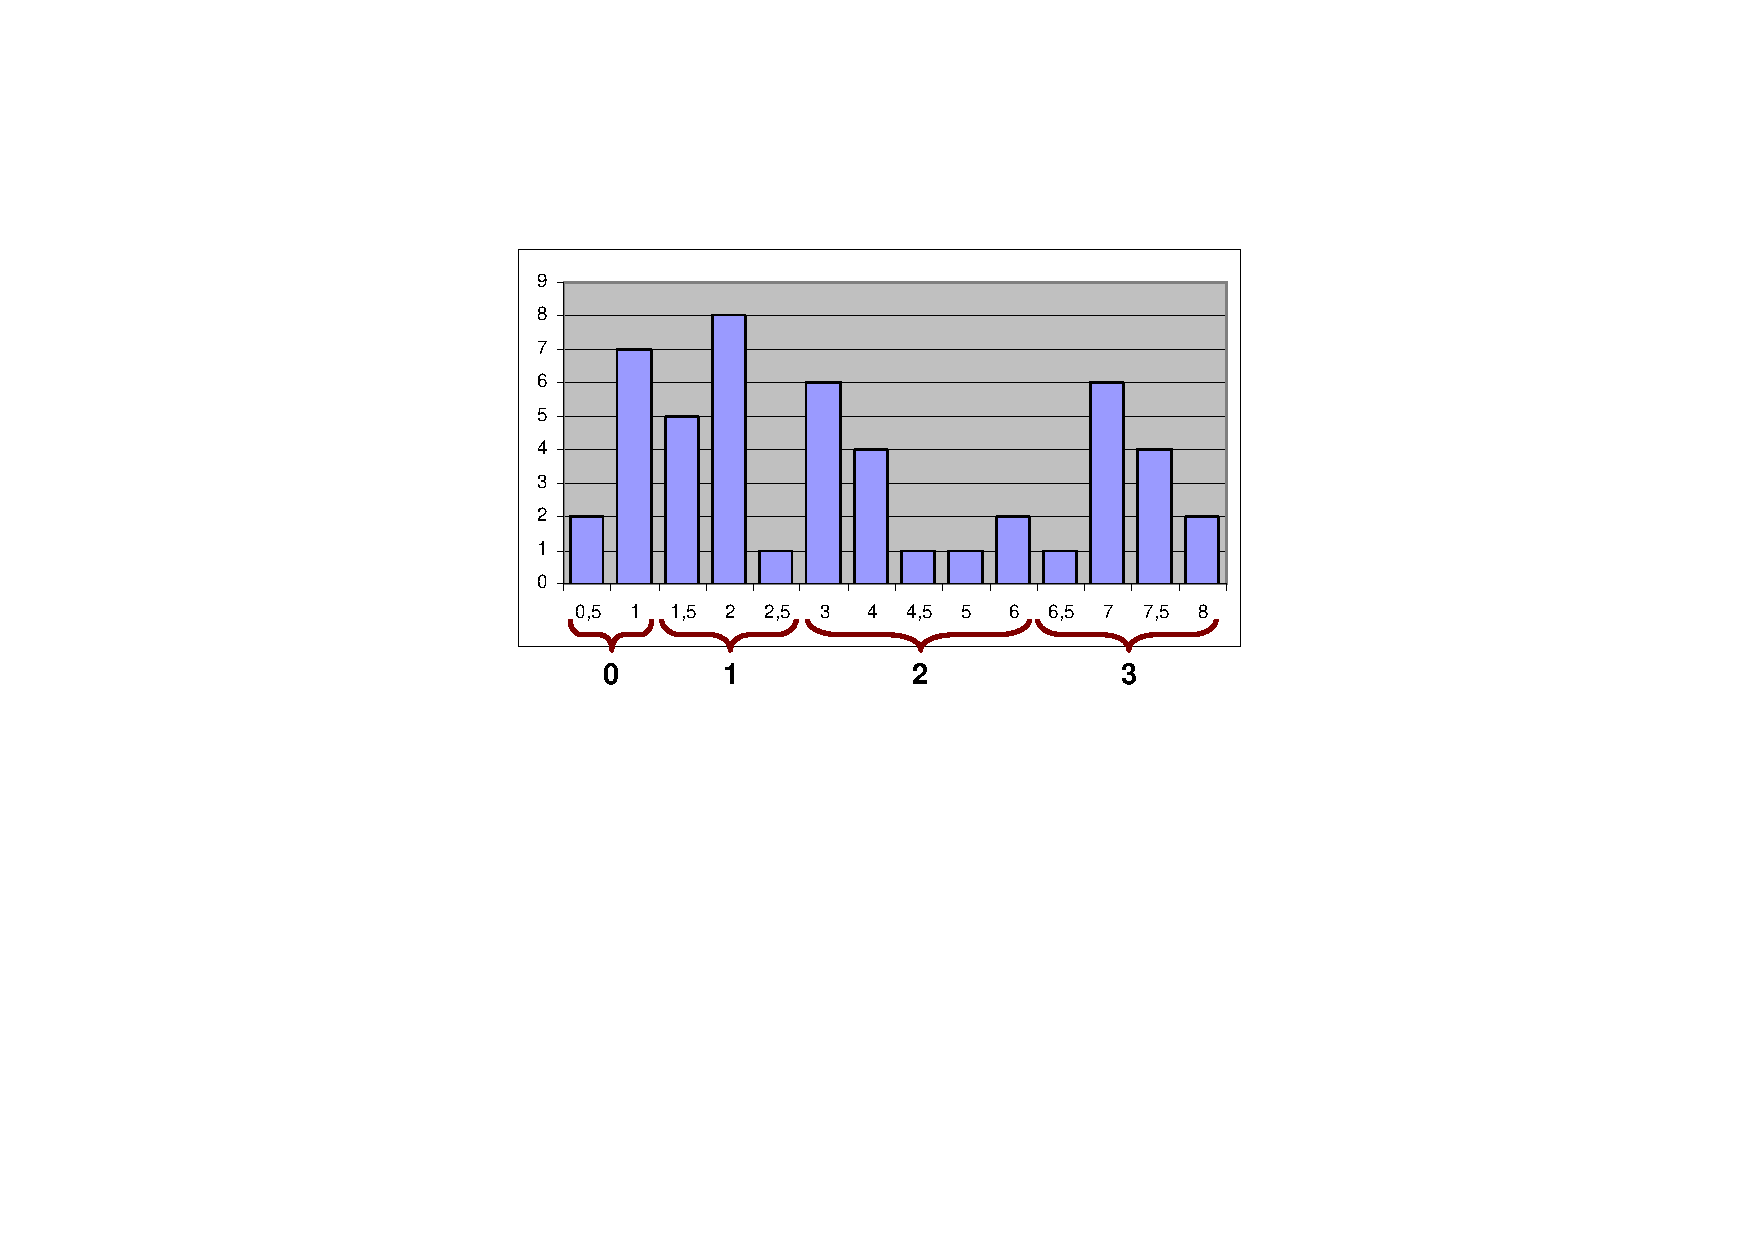
\includegraphics[angle=-90, width=0.6\hsize]{ranking_histogram}}
\caption{Frequencies of the seriousness ranking.}
\label{img:ranking_histogram}
\end{figure}

Values of the overall seriousness ranking attribute were stated from ``a general impression'' made by the texts with respect to particular attributes. %(Fig.~\ref{img:attributes_description}). 
The values have evolved to 14 distinct values in the range from 0.5 to 8. 
A histogram with frequencies of all these values is in Figure~\ref{img:ranking_histogram}.
We have divided the values into four approximately equipotent groups 
(see in Fig.~\ref{img:ranking_histogram}) 
and these groups determine the target class attribute of the classification task. 
%and logic rules were learned for each group separately\footnote{We do not have a binary rule, which would return an exact value of the rating, but we have one ``true/false'' rule for each of the four categories.}.








%%%%%%%%%%%%%%%%%%%%%%%%%%%%%%%%%%%%%%%%%%%%%%%%%%%%%%%%%%%%%%%%%%%%%%%%%%%%%%%%%%%%%%%%%%%%%%%%%
\section{ILP models and methods} \label{sec:ILP}
%%%%%%%%%%%%%%%%%%%%%%%%%%%%%%%%%%%%%%%%%%%%%%%%%%%%%%%%%%%%%%%%%%%%%%%%%%%%%%%%%%%%%%%%%%%%%%%%%






To make the text easier to read, we present a short description of the ILP techniques below.

%%%%%%%%%%%%%%%%%%%%%%%%%%%%%%%%%%%%%%%%%%%%%%%%%%%%%%%%%%%%%%%%%%%%%%%%%%%%%%%%%%%%%%%%%%%%%%%%%
\subsection{Classical ILP}
%%%%%%%%%%%%%%%%%%%%%%%%%%%%%%%%%%%%%%%%%%%%%%%%%%%%%%%%%%%%%%%%%%%%%%%%%%%%%%%%%%%%%%%%%%%%%%%%%

In our presentation of ILP we follow \cite{dzeroski2001:relat_dm} and  \cite{biblio:Muggleton94inductivelogic}.


\theoremstyle{definition}
\newtheorem{definition}{Definition}
\newtheorem{theorem}{Theorem}

\begin{definition}[Classical ILP task]
A set of examples $E=P\cup N$, where $P$ contains positive and $N$ negative examples, and background knowledge denoted by $B$ are given. The task of ILP is to find a hypothesis $H$ such that 

$$
(\forall e\in P)(B\cup H\models e)
$$
and
$$
(\forall e\in N)(B\cup H\not\models e).
$$
\end{definition}
Typically, $E$ consists of ground instances of the target predicate, in our case accident seriousness (see examples in Fig.~\ref{img:examples}). $B$ typically consists of several predicates (relational tables), which describe properties of an object, in our case properties of an accident (see examples in Fig.~\ref{img:crisp_attributes}). The background knowledge can also contain some rules. A hypothesis $H$ typically consists of logic programming rules (see examples in Fig.~\ref{img:rules}). $H$ added to $B$ entails all positive examples and no negative examples.
%
The main advantage of ILP is its multirelational character, namely, $B$ can reside in several relational tables.





%%%%%%%%%%%%%%%%%%%%%%%%%%%%%%%%%%%%%%%%%%%%%%%%%%%%%%%%%%%%%%%%%%%%%%%%%%%%%%%%%%%%%%%%%%%%%%%%%
\subsection{Fuzzy and GAP induction}
%%%%%%%%%%%%%%%%%%%%%%%%%%%%%%%%%%%%%%%%%%%%%%%%%%%%%%%%%%%%%%%%%%%%%%%%%%%%%%%%%%%%%%%%%%%%%%%%%

In our presentation of fuzzy ILP we follow the paper of T. Horv\'ath and P. Vojt\'a\v s \citep{biblio:FILP} about fuzzy inductive logic programming.
We use the approach of the fuzzy logic in a narrow sense, developed by J.~Pavelka \citep{biblio:Pavelka} and P. H\'ajek \citep{biblio:Hajek}. Formulas are of the form $\varphi, x$ ($\varphi$ is syntactically the same as in the classical case), they are graded by a truth value $x\in [0,1]$.
A structure ${\mathcal M}$ consists of a domain $M$ and relations are interpreted as fuzzy (we do not consider function symbols here). The evaluation $\left\|\varphi\right\|_{{\mathcal M}}$ of a formula $\varphi$ uses truth functions of many-valued connectives (our logic is extensional and/or truth functional). The satisfaction $\models_f$ is defined by
$$
{\mathcal M}\models_f (\varphi, x)\ iff\ \left\|\varphi\right\|_{{\mathcal M}}\ge x.
$$

\begin{definition}[Fuzzy ILP task]
A fuzzy set of examples ${\mathcal E}:E\longrightarrow [0,1]$ and a fuzzy background knowledge ${\mathcal B}:B\longrightarrow [0,1]$ are given. The task of fuzzy ILP is to find a fuzzy hypothesis ${\mathcal H}:H\longrightarrow [0,1]$ such that 

$$
(\forall e_1,e_2\in E)(\forall {\mathcal M})({\mathcal M}\models_f {\mathcal B}\cup {\mathcal H})
$$
we have
$$
{\mathcal E}(e_1)>{\mathcal E}(e_2)\Rightarrow \left\|e_1\right\|_{{\mathcal M}}\ge \left\|e_2\right\|_{{\mathcal M}}.
$$
That is, it cannot happen that
$$
{\mathcal E}(e_1)>{\mathcal E}(e_2) \wedge \left\|e_1\right\|_{{\mathcal M}}< \left\|e_2\right\|_{{\mathcal M}},
$$
or rephrased: if ${\mathcal E}$ is rating $e_1$ higher than $e_2$, then it cannot happen that $e_1$ is rated worse than $e_2$ in a model of ${\mathcal B}\cup {\mathcal H}$.
\end{definition}

Typically, ${\mathcal E}$ consists of ground instances of the target predicate, which are classified in truth degrees, in our case degrees of seriousness of an accident. ${\mathcal B}$ typically consists of several fuzzy predicates (fuzzy relational tables), which describe properties of an object, in our case fuzzy properties of an accident -- a degree of injury, a degree of damage, etc. 
%Background knowledge can contain also some rules, so far only crisp rules are used.
A~hypothesis ${\mathcal H}$ typically consists of a fuzzy logic program, which, when added to ${\mathcal B}$, prevents misclassification (what is better cannot be declared to be worse, nevertheless it can be declared as having the same degree -- for more detailed discussion on this definition of fuzzy ILP we refer to the paper \citep{biblio:FILP}).

Moreover, we use GAP -- Generalized Annotated Programs -- in practice, so graded formulas will sometimes be understood as annotated (with classical connectives and with a more complex annotation of the heads of rules). This is possible because in \citep{biblio:KLV} we have shown that (some extension of) fuzzy logic programming is equivalent to (some restriction of) generalized annotated programs. 



%%%%%%%%%%%%%%%%%%%%%%%%%%%%%%%%%%%%%%%%%%%%%%%%%%%%%%%%%%%%%%%%%%%%%%%%%%%%%%%%%%%%%%%%%%%%%%%%%
\subsection{Translation of fuzzy ILP task to several classical ILP tasks}
%%%%%%%%%%%%%%%%%%%%%%%%%%%%%%%%%%%%%%%%%%%%%%%%%%%%%%%%%%%%%%%%%%%%%%%%%%%%%%%%%%%%%%%%%%%%%%%%%

As far as there is no implementation of fuzzy ILP or GAP, we have to use a~classical ILP system. Fortunately, any fuzzy ILP task can be translated to several classical ILP tasks (subject to some rounding and using a finite set of truth values).

In the following text, assume that all fuzzy sets take truth values only from a finite set of truth values $T: \{0,1\}\subseteq T\subseteq [0,1]$.

\begin{definition}[Transformation of background knowledge]
A fuzzy background knowledge ${\mathcal B}:B\longrightarrow [0,1]$ is given. For each predicate $p(x)$ in $B$ we insert an additional attribute $t$ to express the truth value, thus we have created a new predicate $p(x,t)$. We construct two classical background knowledge sets $B^{raw}_T$ and $B^{mon}_T$  as follows:

\begin{itemize}
	\item The first ($B^{raw}_T$) is a direct coding of a fuzzy value by an additional attribute:
\\If ${\mathcal B}(p(x))=t,\  t \in T$, then we add $p(x,t)$ to  ${B}^{raw}_T$.
	\item The second ($B^{mon}_T$) is obtained by a process called monotonization:
\\If ${\mathcal B}(p(x))=t,\  t \in T$, then for all $t'\in T,\  t'\le t$ we add $p(x,t')$ to ${B}^{mon}_T$.
This corresponds to the natural meaning of truth values $t$.
\end{itemize}
\end{definition}



Additionally, example sets are constructed in two ways.
\begin{definition}[Transformation of examples]
Given is a fuzzy set of examples ${\mathcal E}:E\longrightarrow [0,1]$. For all $t\in T$ we construct two classical sets of examples $E_t$ and $E_{\ge t}$  as follows:
\begin{itemize}
	\item $E_t=P_t\cup N_t$, where 
$e\in P_t \ \ iff \ \ {\mathcal E}(e)= t$
and $N_t$ is the rest of $E$.
	\item $E_{\ge t}=P_{\ge t}\cup N_{\ge t}$, where 
$e\in P_{\ge t} \ \ iff \ \ {\mathcal E}(e)\ge t$
and $N_t$ is the rest of $E$.
\end{itemize}
\end{definition}



These two translations create two classical ILP tasks for each truth value $t\in T$, the first one (\emph{raw}) is crisp and the second one (\emph{mon}) can be understood as (and translated back to) fuzzy ILP.

\begin{itemize}
	\item The \textit{raw ILP task} is given by $B^{raw}_{T}$ and $E_t$ for each $t\in T$.  As a~result, it produces a set of hypotheses $H_t$.

	\item The \textit{mon ILP task} is given by ${B}^{mon}_T$ and $E_{\ge t}$ for each $t\in T$. As a~result, it produces a set of hypotheses $H_{\ge t}$ guaranteeing examples of a degree of at least $t$.
\end{itemize}

Note that among variable boundings in $B$ there are no boundings on the truth value attribute which was added to each predicate; hence, there are no variable boundings on the truth value attribute in $H_{\ge t}$. We did not add an additional truth value attribute to the predicates in $E$. 

Now we sketch the translation of the \emph{mon ILP task} to GAP (fuzzy ILP) rules. 

\begin{theorem}[Translation of the \emph{mon ILP task}]
A fuzzy ILP (or equivalent GAP) task is given by ${\mathcal E}$ and ${\mathcal B}$. Let us assume that $C$ is the target predicate in the domain of ${\mathcal E}$ and for each $t \in T$, $H_{\ge t}$ is a correctly learned solution of the corresponding \textit{mon ILP task} according to the definitions introduced above. We define ${\mathcal H}$ consisting of one GAP rule:
$$C(y):u(x_1,\dots,x_m)\leftarrow B_1(y):x_1\; \&\dots\& \;B_m(y):x_m,$$
here $B_1:x_1 \&\dots\& B_m:x_m$ is the enumeration of all predicates in $B$.

Assume that $B_1(y_1,t_1),\dots,B_n(y_n,t_n)$ are some of the predicates in $B$ (for simplicity enumerated from 1 to $n, \ n \le m$). Then for each rule 
$$
R=C_{\ge t}(y)\Leftarrow B_1(y,t_1),\dots,B_n(y,t_n)
$$
in $H_{\ge t}$ ($C_{\ge t}$ is the monotonized target predicate) we give a constraint in the definition of $u$ as follows:
$$
U_R=u(x_1,\dots,x_m)\ge t \hbox{ if }x_1\ge t_1,\dots,x_n\ge t_n.
$$
Note that all $x_i$ and $y$ are variables, $t_i$ and $t$ are constants and $x_{n+1},\dots,x_m$ have no restrictions.
We learn the function $u$ as a ``monotone'' completion of the rules. 

We claim that if all $H_{\ge t}$ were correctly learned by a classical ILP system, then, for the minimal solution $u$ of all constraints $U_R$, the rule
$$
C(y):u(x_1,\dots,x_m)\leftarrow B_1(y):x_1\; \&\dots\& \;B_m(y):x_m
$$
is a correct solution of the fuzzy ILP task given by ${\mathcal E}$ and ${\mathcal B}$, for all $R\in H_{\ge t}$ and $t\in T$. 
\end{theorem}

In our case \verb@serious(Accident_ID)@ is the fuzzy or GAP target predicate $C$. Let for example $t=3$ and $H_{\ge t}$ is the same as in Fig.~\ref{img:rules} (the last two rows correspond with $H_{\ge 3}$). Then \verb@serious_atl_3(Accident_ID)@ is the monotonized target predicate $C_{\ge t}$ and $B_1$, $B_2$ and $u$ are realized as follows:\\
\hspace*{1cm}$B_1(y,t_1)$ \dots \verb@fatalities_atl(Accident_ID, 1)@,\\
\hspace*{1cm}$B_2(y,t_2)$ \dots \verb@damage_atl(Accident_ID, 1500000)@,\\
$u$ is an arbitrary function of $m$ arguments ($m$ is the number of all predicates used in background knowledge) for which following restrictions hold true:\\
for $t=3$:\\
\hspace*{1cm}$u(x_1,\dots,x_m) \ge 3 \ \hbox{ if }x_1\ge 1$\\
\hspace*{1cm}$u(x_1,\dots,x_m) \ge 3 \ \hbox{ if }x_2\ge 1500000$\\
and similar restrictions for $t=1,2$.


\bigskip
Our presentation is slightly simplified here and we freely switch between fuzzy and GAP programs, which are known to be equivalent, see in~\citep{biblio:KLV}.


%%%%%%%%%%%%%%%%%%%%%%%%%%%%%%%%%%%%%%%%%%%%%%%%%%%%%%%%%%%%%%%%%%%%%%%%%%%%%%%%%%%%%%%%%%%%%%%%%
\subsection{Implementation} \label{sec:implementation}
%%%%%%%%%%%%%%%%%%%%%%%%%%%%%%%%%%%%%%%%%%%%%%%%%%%%%%%%%%%%%%%%%%%%%%%%%%%%%%%%%%%%%%%%%%%%%%%%%

In our experimental system we use two inductive logic approaches: crisp and fuzzy (as described above). Technically, the difference between the approaches consists in a different setting of the \emph{ILP task}. Both can be done with a classical ILP tool. We have used 
``\emph{A Learning Engine for Proposing Hypotheses}'' (Aleph  v5\footnote{\url{http://www.comlab.ox.ac.uk/activities/machinelearning/Aleph/}}), which we consider very practical. It uses the quite effective method of \emph{inverse entailment} \citep{biblio:InverseEntailment} and keeps all handy features of a Prolog system (it is supported by YAP and SWI Prolog) in its background.

We have compared results of the crisp and fuzzy approaches with other classification methods and, in our experiment, the fuzzy approach produced better results than many other methods, including the crisp one. See Section~\ref{sec:results} for details.



\begin{figure}
\begin{minipage}[b]{0.5\hsize}
	Crisp learning examples\\
\begin{minted}[fontsize=\footnotesize,
               frame=single]{prolog}
serious_2(id_47443). %positive

serious_0(id_47443). %negative
serious_1(id_47443). %negative
serious_3(id_47443). %negative							
\end{minted}						
	Monotonized learning examples\\
\begin{minted}[fontsize=\footnotesize,
               frame=single]{prolog}
serious_atl_0(id_47443). %positive
serious_atl_1(id_47443). %positive
serious_atl_2(id_47443). %positive

serious_atl_3(id_47443). %negative					
\end{minted}						
	\caption{Learning examples.}
	\label{img:examples}
\end{minipage}
\hspace{0.5cm}
\begin{minipage}[b]{0.5\hsize}
\begin{minted}[fontsize=\footnotesize,
               frame=single]{prolog}
size(id_47443, 427).
type(id_47443, fire).
damage(id_47443, 8000).
dur_minutes(id_47443, 50).
fatalities(id_47443, 0).
injuries(id_47443, 0).
cars(id_47443, 0).
amateur_units(id_47443, 3).
profesional_units(id_47443, 1).
pipes(id_47443, unknown).
lather(id_47443, 0).
aqualung(id_47443, 0).
fan(id_47443, 0).
\end{minted}						
	\caption{$B^{raw}_{T}$ -- crisp attributes.}
	\label{img:crisp_attributes}
\end{minipage}
\end{figure}

\begin{figure}[htb]	
\begin{minted}[fontsize=\footnotesize,
               frame=lines]{prolog}
damage_atl(ID,N) :- damage(ID,N), not(integer(N)). %unknown values

damage_atl(ID,N) :- damage(ID,N2), integer(N2), %numeric values
                    damage(N), integer(N), N2>=N.
\end{minted}						
	\caption{Monotonization of attributes (damage\_atl $\leftarrow$ damage).}
	\label{img:attribute_monotonization}
\end{figure}

\begin{figure}[htb]	
\begin{minted}[fontsize=\footnotesize,
               frame=lines]{prolog}
serious_0(ID) :- serious_atl_0(ID),
                 not(serious_atl_1(ID)), not(serious_atl_2(ID)), not(serious_atl_3(ID)).
serious_1(ID) :- serious_atl_1(ID),
                 not(serious_atl_2(ID)), not(serious_atl_3(ID)).
serious_2(ID) :- serious_atl_2(ID),
                 not(serious_atl_3(ID)).
serious_3(ID) :- serious_atl_3(ID).
\end{minted}						
\caption{Conversion rules for monotonized hypotheses (\texttt{serious\_t} $\leftarrow$ \texttt{serious\_atl\_t}).}
\label{img:conversion}
\end{figure}





To use ILP for a classification task we have to translate the input data to the Prolog-like logic representation, as it was already described in previous sections. Here we will describe implementation details of constructing crisp and fuzzy knowledge bases and example sets.

In construction of a crisp example set $E_t$, the target predicate is denoted as \texttt{serious\_t}. The letter \texttt{t} stands for the actual seriousness degree. We use multiple unary predicates \texttt{serious\_0}, \texttt{serious\_1}, etc., instead of one binary predicate \texttt{serious(ID,Degree)}. These two cases are equivalent and we have decided to use the unary option because a visual distinction between the multiple ILP tasks is then clearer.

In construction of a fuzzy (or monotonized) example set $E_{\ge t}$, the target predicate is denoted as \texttt{serious\_atl\_t}, see examples in Fig.~\ref{img:examples}.



In construction of a crisp background knowledge $B^{raw}_{T}$, we use a~simple translation of the attribute names to the names of predicates and fill them with actual values. It is illustrated in Fig.~\ref{img:crisp_attributes}). 



In construction of a monotonized background knowledge $B^{mon}_T$ we reuse the crisp background knowledge and add monotonization rules. An~example for predicate \texttt{damage} is shown in Fig.~\ref{img:attribute_monotonization}.
%on predicates \texttt{damage} and \texttt{damage\_atl}.
The first rule deals with \texttt{unknown} values and the second does the monotonization. 

Negations used in Fig.~\ref{img:attribute_monotonization} and Fig.~\ref{img:conversion} are the standard Prolog \emph{negations as failure}.


\begin{figure}[bht]
\begin{minted}[linenos,  fontsize=\footnotesize,
               frame=lines]{prolog}
serious_0(A) :- fatalities(A,0), injuries(A,0), cars(A,1), amateur_units(A,0), lather(A,0).
serious_0(A) :- fatalities(A,0), cars(A,0), amateur_units(A,0), professional_units(A,1).
serious_1(A) :- amateur_units(A,1).
serious_1(A) :- damage(A,300000).
serious_1(A) :- type(A,fire), amateur_units(A,0), pipes(A,2).
serious_1(A) :- type(A,car_accident),dur_minutes(A,unknown),fatalities(A,0),injuries(A,1).
serious_2(A) :- lather(A,unknown).
serious_2(A) :- cars(A,0), lather(A,0), aqualung(A,1), fan(A,0).
serious_2(A) :- amateur_units(A,2).
serious_3(A) :- fatalities(A,2).
serious_3(A) :- type(A,fire), dur_minutes(A,unknown), cars(A,0), fan(A,0).
serious_3(A) :- injuries(A,2), cars(A,2).
serious_3(A) :- fatalities(A,1).

serious_atl_0(A).
serious_atl_1(A) :- injuries_atl(A,1).
serious_atl_1(A) :- dur_minutes_atl(A,21), pipes_atl(A,1), aqualung_atl(A,0).
serious_atl_1(A) :- damage_atl(A,8000), amateur_units_atl(A,3).
serious_atl_1(A) :- dur_minutes_atl(A,197).
serious_atl_1(A) :- dur_minutes_atl(A,unknown).
serious_atl_2(A) :- dur_minutes_atl(A,50), pipes_atl(A,3).
serious_atl_2(A) :- size_atl(A,1364), injuries_atl(A,1).
serious_atl_2(A) :- fatalities_atl(A,1).
serious_atl_2(A) :- size_atl(A,1106), professional_units_atl(A,3).
serious_atl_3(A) :- fatalities_atl(A,1).
serious_atl_3(A) :- damage_atl(A,1500000).
\end{minted}
\caption{Crisp and monotonized hypotheses.}
\label{img:rules}
\end{figure}


Once we have learning examples and background knowledge, we can run the ILP inductive procedure and obtain learned rules (a learned hypothesis). According to the kind of the ILP task (crisp or monotonized), we obtain the corresponding kind (crisp or monotonized) of rules (see e.g. in Fig.~\ref{img:rules}). But these rules cannot be used directly to solve the classification task. There are common cases when more than one rule is applicable to a single instance. So we have to select which one to use. For the monotonized hypothesis we select the one with the biggest return value. It is illustrated in Fig.~\ref{img:conversion}. Such clear criterion does not exist for the crisp hypothesis, so we simply use the first applicable rule.


In the crisp case there are often many instances which cannot be classified because there is no applicable rule. In our experiment there was about a 51\%
of unclassified instances (see in the next section). It could be caused by the lack of training data, but the monotonized approach does not suffer from this shortage. We can always select the bottom value.

Another advantage of the monotonized approach is that the set of positive training examples is extended by monotonization. 





%%%%%%%%%%%%%%%%%%%%%%%%%%%%%%%%%%%%%%%%%%%%%%%%%%%%%%%%%%%%%%%%%%%%%%%%%%%%%%%%%%%%%%%%%%%%%%%%%
\section{Results} \label{sec:results}
%%%%%%%%%%%%%%%%%%%%%%%%%%%%%%%%%%%%%%%%%%%%%%%%%%%%%%%%%%%%%%%%%%%%%%%%%%%%%%%%%%%%%%%%%%%%%%%%%

Fig.~\ref{img:rules} summarizes obtained hypotheses learned from our data: 
\begin{itemize}
	\item a crisp hypothesis learned from $E_t$ and $B^{raw}_{T}$ and
	\item a monotonized hypothesis learned from $E_{\ge t}$ and ${B}^{mon}_T$.
\end{itemize}


In both cases, learning examples and background knowledge have the origin in the same data (the same accidents). The hypotheses differ in the form of the ILP task (crisp and monotonized). The crisp hypothesis uses only the crisp predicates, and the monotonized hypothesis uses only the monotonized predicates.


%%%%%%%%%%%%%%%%%%%%%%%%%%%%%%%%%%%%%%%%%%%%%%%%%%%%%%%%%%%%%%%%%%%%%%%%%%%%%%%%%%%%%%%%%%%%%%%%%
\subsection{Evaluation} \label{sec:ch80_eval}
%%%%%%%%%%%%%%%%%%%%%%%%%%%%%%%%%%%%%%%%%%%%%%%%%%%%%%%%%%%%%%%%%%%%%%%%%%%%%%%%%%%%%%%%%%%%%%%%%

\begin{figure}[p]
\centerline{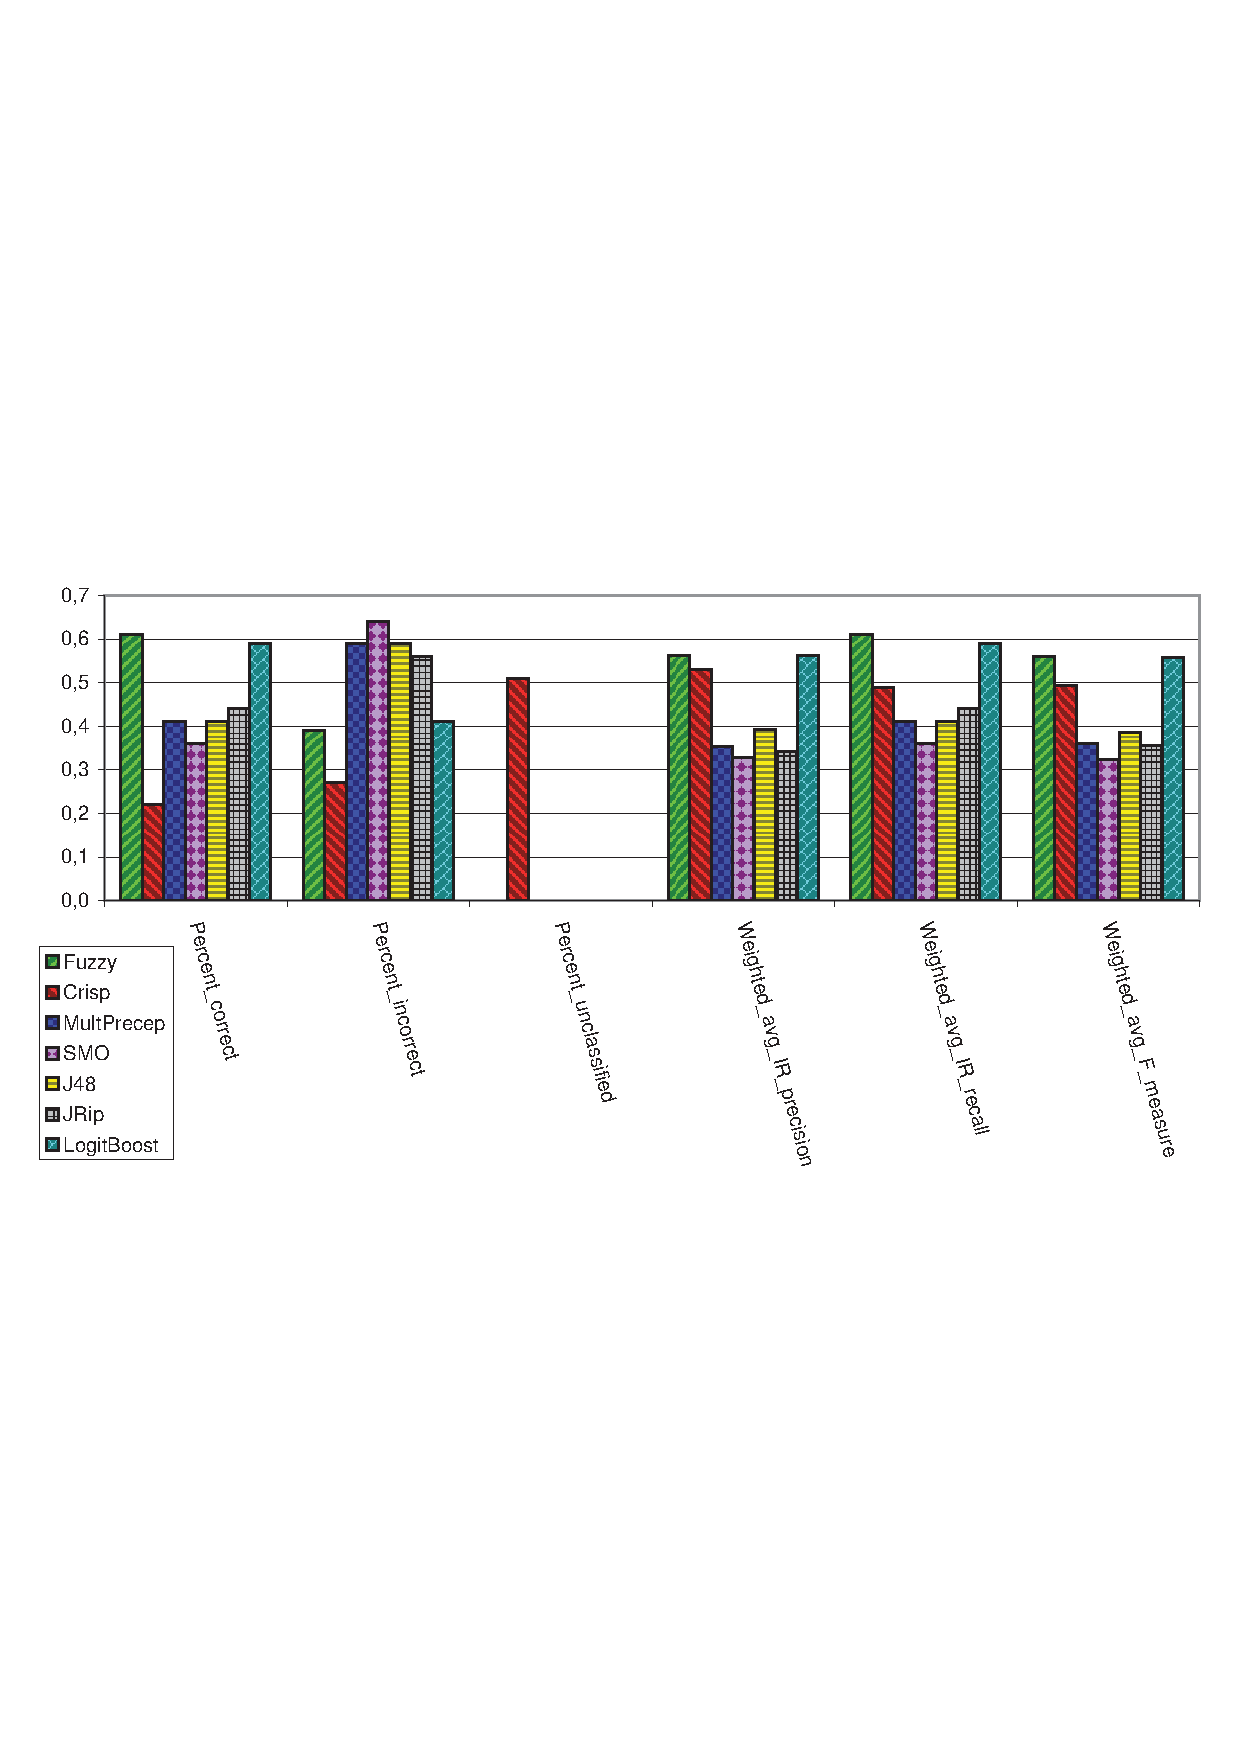
\includegraphics[width=0.8\hsize]{2x10cross}}
\caption{Evaluation of the methods -- average values.}
\label{img:graph2x10}
\end{figure}


\begin{table}[p]
\scriptsize
{\centering \begin{tabular}{lr@{\hspace{0cm}}c@{\hspace{0cm}}rr@{\hspace{0cm}}c@{\hspace{0cm}}r@{\hspace{0.05cm}}cr@{\hspace{0cm}}c@{\hspace{0cm}}r@{\hspace{0.05cm}}cr@{\hspace{0cm}}c@{\hspace{0cm}}r@{\hspace{0.05cm}}cr@{\hspace{0cm}}c@{\hspace{0cm}}r@{\hspace{0.05cm}}cr@{\hspace{0cm}}c@{\hspace{0cm}}r@{\hspace{0.05cm}}cr@{\hspace{0cm}}c@{\hspace{0cm}}r@{\hspace{0.05cm}}c}
\hline
& \multicolumn{3}{c}{Fuzzy}& \multicolumn{4}{c}{Crisp} & \multicolumn{4}{c}{MultPerc} & \multicolumn{4}{c}{SMO} & \multicolumn{4}{c}{J48} & \multicolumn{4}{c}{JRip} & \multicolumn{4}{c}{LBoost} \\
\hline
Corr	& 0.61 & $\pm$ & .19 & .22 & $\pm$ & .17 & $\bullet$ & .41 & $\pm$ & .19 & $\bullet$ & .36 & $\pm$ & .24 & $\bullet$ & .41 & $\pm$ & .22 & $\bullet$ & .44 & $\pm$ & .17 & $\bullet$ & .59 & $\pm$ & .26 &        \\
Incor	&  .39 & $\pm$ & .19 & .27 & $\pm$ & .24 &         	 & .59 & $\pm$ & .19 & $\circ$ 	 & .64 & $\pm$ & .24 & $\circ$ 	 & .59 & $\pm$ & .22 & $\circ$ 	 & .56 & $\pm$ & .17 & $\circ$ 	 & .41 & $\pm$ & .26 &        \\
Uncl	&  .00 & $\pm$ & .00 & .51 & $\pm$ & .29 & $\circ$   & .00 & $\pm$ & .00 &         	 & .00 & $\pm$ & .00 &         	 & .00 & $\pm$ & .00 &         	 & .00 & $\pm$ & .00 &         	 & .00 & $\pm$ & .00 &        \\
Prec	&  .56 & $\pm$ & .24 & .53 & $\pm$ & .37 &         	 & .35 & $\pm$ & .20 & $\bullet$ & .33 & $\pm$ & .26 &         	 & .39 & $\pm$ & .22 &         	 & .34 & $\pm$ & .21 & $\bullet$ & .56 & $\pm$ & .28 &        \\
Rec		&  .61 & $\pm$ & .19 & .49 & $\pm$ & .32 &         	 & .41 & $\pm$ & .19 & $\bullet$ & .36 & $\pm$ & .24 & $\bullet$ & .41 & $\pm$ & .22 & $\bullet$ & .44 & $\pm$ & .17 & $\bullet$ & .59 & $\pm$ & .26 &        \\
F			&  .56 & $\pm$ & .20 & .49 & $\pm$ & .33 &         	 & .36 & $\pm$ & .19 & $\bullet$ & .32 & $\pm$ & .24 & $\bullet$ & .39 & $\pm$ & .21 &         	 & .36 & $\pm$ & .19 & $\bullet$ & .56 & $\pm$ & .27 &        \\
\hline
\multicolumn{21}{c}{$\circ$, $\bullet$ statistically significant increase or decrease}\\
\end{tabular} \scriptsize \par}
\scriptsize
\smallskip
Legend:\\
{\centering
\begin{tabular}{p{2cm}@{}p{10.5cm}}\\
Fuzzy \dotfill{}& czsem.ILP.FuzzyILPClassifier '' \\
Crisp \dotfill{} & czsem.ILP.CrispILPClassifier '' \\
MultPerc \dotfill{} & functions.MultilayerPerceptron '-L 0.3 -M 0.2 -N 500 -V 0 -S 0 -E 20 -H a' \\
SMO \dotfill{} & functions.SMO '-C 1.0 -L 0.0010 -P 1.0E-12 -N 0 -V -1 -W 1 -K \textbackslash"functions.supportVector.PolyKernel -C 250007 -E 1.0\textbackslash"' \\
J48 \dotfill{} & trees.J48 '-C 0.25 -M 2' \\
JRip \dotfill{} & rules.JRip '-F 3 -N 2.0 -O 2 -S 1' \\
LBoost \dotfill{} & meta.LogitBoost '-P 100 -F 0 -R 1 -L -1.7976931348623157E308 -H 0.1 -S 1 -I 10 -W trees.DecisionStump' \\
\\
Corr \dotfill{} & Percent correct\\
Inor \dotfill{} & Percent incorrect\\
Uncl \dotfill{} & Percent unclassified\\
Prec \dotfill{} & IR precision, weighted average from all classes\\
Rec \dotfill{} 	& IR recall, weighted average from all classes\\
F \dotfill{} 		& F measure, weighted average from all classes\\
\end{tabular}
}
\caption{Evaluation of the methods in 2 times 10-fold cross validation.}
\label{tab:table2x10}
\end{table}


We have evaluated both ILP methods and compared them with other machine learning procedures used in data mining. To make the comparison clear and easy to perform, we have implemented an interface between the ILP methods and the Weka data mining software\footnote{\url{http://www.cs.waikato.ac.nz/ml/weka/}} \citep{biblio:Weka}. This interface makes it possible to use the ILP methods as an ordinary Weka classifier for any\footnote{For the fuzzy ILP method, there is a requirement on the target (class) attribute: it has to be monotonizable (e.g. numeric).} classification task inside the Weka software. Our implementation is publicly available. The data, source codes and a platform-independent installer of the Crisp and Fuzzy ILP classifiers for Weka can be downloaded from our Fuzzy ILP classifier's web page\footnote{\url{http://www.ksi.mff.cuni.cz/~dedek/fuzzyILP/}}. This makes our experiment repeatable according to the
SIGMOD Experimental Repeatability Requirements \citep{biblio:SIGMODrepeatability}.


For our experiment we used the Weka Experimenter and performed an experiment in which the Crisp and Fuzzy ILP classifiers were compared with five additional classifiers:
\begin{itemize}
	\item Multilayer Perceptron \citep{biblio:bishop-1995},
	\item Support Vector Machine classifier SMO \citep{biblio:SMO},
	\item J48 decision tree \citep{biblio:J48},
	\item JRip rules \citep{weka:JRip} and
	\item Additive logistic regression LogitBoost \citep{biblio:LogitBoost}.
\end{itemize}
We have evaluated all the methods two times by 10-fold cross validation. %(section~\ref{sec:experiment_desc}).
The obtained results (average values) are described by the graph in Fig.~\ref{img:graph2x10} and in Table~\ref{tab:table2x10} (with standard deviations and marked statistically significant values).

There is no clear winner in our experiment. But the Fuzzy ILP classifier proved better results than a majority of the methods on our data and the results are statistically significant in many cases. Very good results were also obtained using LogitBoost. 


%%%%%%%%%%%%%%%%%%%%%%%%%%%%%%%%%%%%%%%%%%%%%%%%%%%%%%%%%%%%%%%%%%%%%%%%%%%%%%%%%%%%%%%%%%%%%%%%%%
\subsubsection*{UCI datasets}
%%%%%%%%%%%%%%%%%%%%%%%%%%%%%%%%%%%%%%%%%%%%%%%%%%%%%%%%%%%%%%%%%%%%%%%%%%%%%%%%%%%%%%%%%%%%%%%%%%



\begin{table}[th!]
\scriptsize
{\centering \begin{tabular}{l|r@{\hspace{0cm}}c@{\hspace{0cm}}r@{\hspace{0.3cm}}r@{\hspace{0cm}}c@{\hspace{0cm}}r@{\hspace{0.05cm}}cr@{\hspace{0cm}}c@{\hspace{0cm}}r@{\hspace{0.05cm}}l@{\hspace{0cm}}r@{\hspace{0cm}}c@{\hspace{0cm}}r@{\hspace{0.05cm}}cr@{\hspace{0cm}}c@{\hspace{0cm}}r@{\hspace{0.05cm}}cr@{\hspace{0cm}}c@{\hspace{0cm}}r@{\hspace{0.05cm}}cr@{\hspace{0cm}}c@{\hspace{0cm}}r@{\hspace{0cm}}c@{\hspace{0.25cm}}c@{\hspace{0.20cm}}c@{\hspace{0.10cm}}}
& \multicolumn{3}{c}{Fuzzy}& \multicolumn{4}{c}{Crisp} & \multicolumn{4}{c}{MultPerc} & \multicolumn{4}{c}{SMO} & \multicolumn{4}{c}{J48} & \multicolumn{4}{c}{JRip} & \multicolumn{4}{c}{LBoost} & train & test\\
\hline
car & .39 & $\pm$ & .03 & .36 & $\pm$ & .03 & $\bullet$ & .53 & $\pm$ & .02 & $\circ$ & .57 & $\pm$ & .01 & $\circ$ & .50 & $\pm$ & .02 & $\circ$ & .51 & $\pm$ & .03 & $\circ$ & .54 & $\pm$ & .02 & $\circ$ & 173 & 1554\\
\hline
wine & .44 & $\pm$ & .03 & .42 & $\pm$ & .02 & $\bullet$ & .48 & $\pm$ & .02 & $\circ$ & .46 & $\pm$ & .02 & $\circ$ & .47 & $\pm$ & .02 & $\circ$ & .48 & $\pm$ & .03 & $\circ$ & .52 & $\pm$ & .02 & $\circ$ & 160 & 1439\\
\hline
cmc & .79 & $\pm$ & .02 & .77 & $\pm$ & .03 & $\bullet$ & .89 & $\pm$ & .02 & $\circ$ & .81 & $\pm$ & .01 & $\circ$ & .88 & $\pm$ & .02 & $\circ$ & .82 & $\pm$ & .03 & $\circ$ & .85 & $\pm$ & .02 & $\circ$ & 147 & 1325\\
\hline
tae & .50 & $\pm$ & .12 & .39 & $\pm$ & .11 & $\bullet$ & .59 & $\pm$ & .11 & $\circ$ & .55 & $\pm$ & .12 & $\circ$ & .50 & $\pm$ & .12 &  & .37 & $\pm$ & .11 & $\bullet$ & .55 & $\pm$ & .11 & $\circ$ & 135 & 15\\
\hline
pop & .66 & $\pm$ & .09 & .54 & $\pm$ & .17 & $\bullet$ & .57 & $\pm$ & .13 & $\bullet$ & .70 & $\pm$ & .06 & $\circ$ & .70 & $\pm$ & .07 & $\circ$ & .70 & $\pm$ & .06 & $\circ$ & .66 & $\pm$ & .10 &  & 80 & 9\\
\hline
nurs & .79 & $\pm$ & .04 & .68 & $\pm$ & .06 & $\bullet$ & .81 & $\pm$ & .04 & $\circ$ & .73 & $\pm$ & .04 & $\bullet$ & .80 & $\pm$ & .04 & $\circ$ & .79 & $\pm$ & .06 &  & .83 & $\pm$ & .02 & $\circ$ & 52 & 12907\\
\hline
\multicolumn{23}{c}{$\circ$, $\bullet$ statistically significant improvement or degradation}\\
\end{tabular} \scriptsize \par}
\scriptsize
\smallskip
Legend:\\
{\centering
\begin{tabular}{p{2cm}@{}p{10.5cm}}\\
train \dotfill{} & average number ($\pm$1) of training instances in each run\\
test \dotfill{} & average number ($\pm$1) of testing instances in each run\\
\\
car \dotfill{} & \url{http://archive.ics.uci.edu/ml/datasets/Car+Evaluation}\\
wine \dotfill{} & red wine dataset \url{http://archive.ics.uci.edu/ml/datasets/Wine+Quality}\\
cmc \dotfill{} & \url{http://archive.ics.uci.edu/ml/datasets/Contraceptive+Method+Choice}\\
tae \dotfill{} & \url{http://archive.ics.uci.edu/ml/datasets/Teaching+Assistant+Evaluation}\\
pop \dotfill{} & \url{http://archive.ics.uci.edu/ml/datasets/Post-Operative+Patient}\\
nurs \dotfill{} & \url{http://archive.ics.uci.edu/ml/datasets/Nursery}\\
\end{tabular}
}


\smallskip


Learning parameters for both ILP methods:\\set(noise,20). set(i,3). set(clauselength,13). set(search,heuristic). set(evalfn,wracc). set(samplesize,3).
\caption{Evaluation of the methods on UCI datasets, \textbf{percent correct}, average values from 100 repetitions.}
\label{tab:UCItable}
\end{table}


The Fuzzy ILP classifier performed quite well on our dataset, but the next question is: How is it with other data, with more learning instances, and what about the time complexity? To answer these questions we performed another experiment. We selected several datasets from the University of California, Irvine, Repository of Machine Learning Databases (UCI) \citep{dedek:UCI} and evaluated all the methods against them. 



The list of selected datasets can be found in the legend of Table~\ref{tab:UCItable}. All the datasets are monotonizable (the target attribute can be naturally ordered), so the fuzzy classifier could take advantage of that. Learning settings are the same as before (Table~\ref{tab:table2x10}) except for settings of both ILP classifiers, which  performed a little bit better with modified settings on a majority of the datasets (see in the legend of Table~\ref{tab:UCItable}). 

Table~\ref{tab:UCItable} compares the numbers of correctly classified instances on all the datasets. The last two columns show numbers of training and testing instances. The numbers of training instances are quite low; this is because the ILP classifiers are probably not capable of fully exploiting higher numbers of training instances and the difference between ILP classifiers and the others would be even a bit higher. This is demonstrated in Fig.~\ref{img:corect_growing_learninig_instances} (for `nursery' dataset only). It can be seen that when the number of training instances was under about 40, the fuzzy classifier performed better than some of the others (SMO, JRip and Multilayer Perceptron), but from about 60 training instances further both ILP classifiers performed worse than the others.


\begin{figure}
\centerline{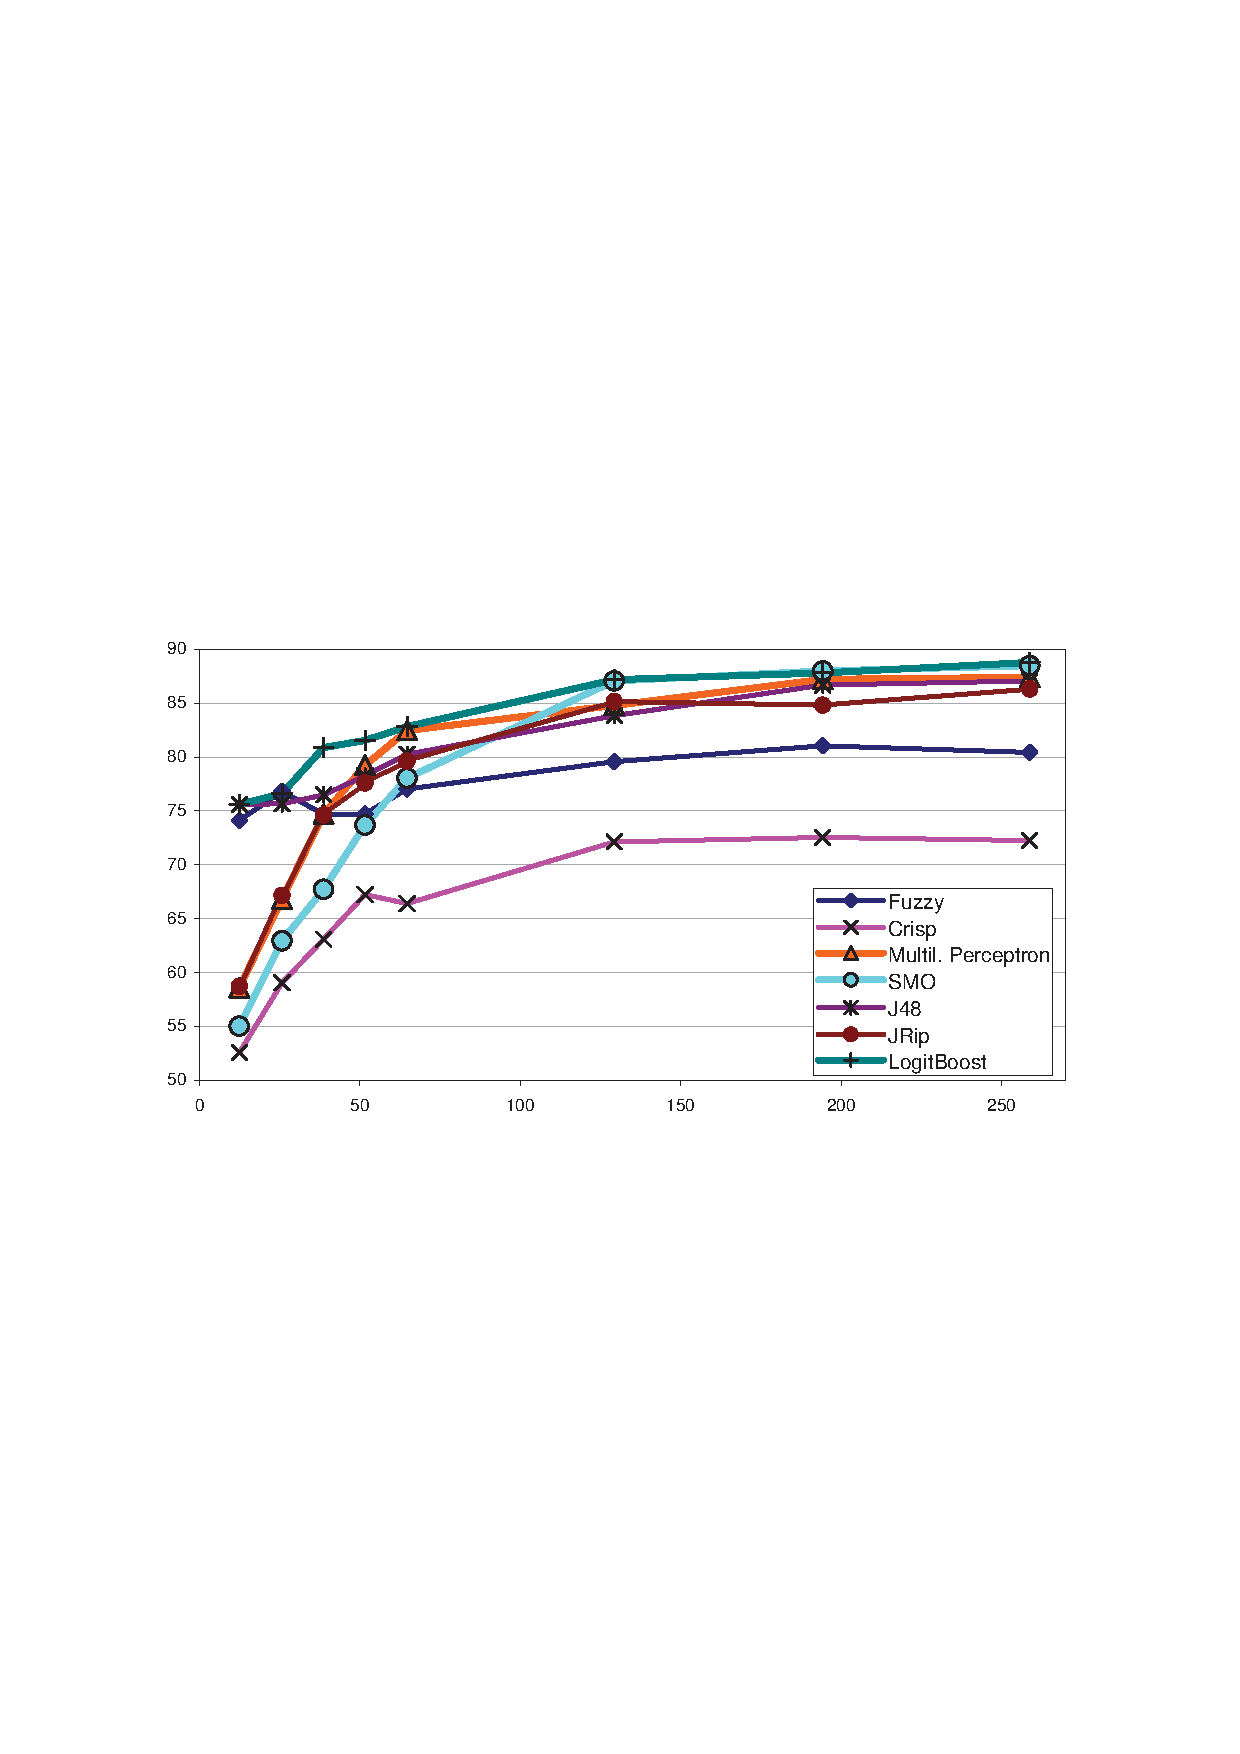
\includegraphics[width=0.8\hsize]{corect_growing_learninig_instances}}
\caption{x-axis: number of training instances, y-axis: percent of correctly classified instances, average values from 10 repetitions, `nursery' dataset.}
\label{img:corect_growing_learninig_instances}
\end{figure}

Fig.~\ref{img:learning_speed} demonstrates time complexity of the classifiers in the same experiment as in Fig.~\ref{img:corect_growing_learninig_instances}. Despite the fact that the Fuzzy ILP classifier was several times slower than the Crisp ILP classifier and even more than the others, it is still computable on current processors (e.g. P9600, 2.66 GHz, which we used) and the curve of time complexity did not grow rapidly during the experiment. Because ILP is a heuristic and iterative method, the time complexity can be quite directly managed by the setting of learning parameters.

\begin{figure}
\centerline{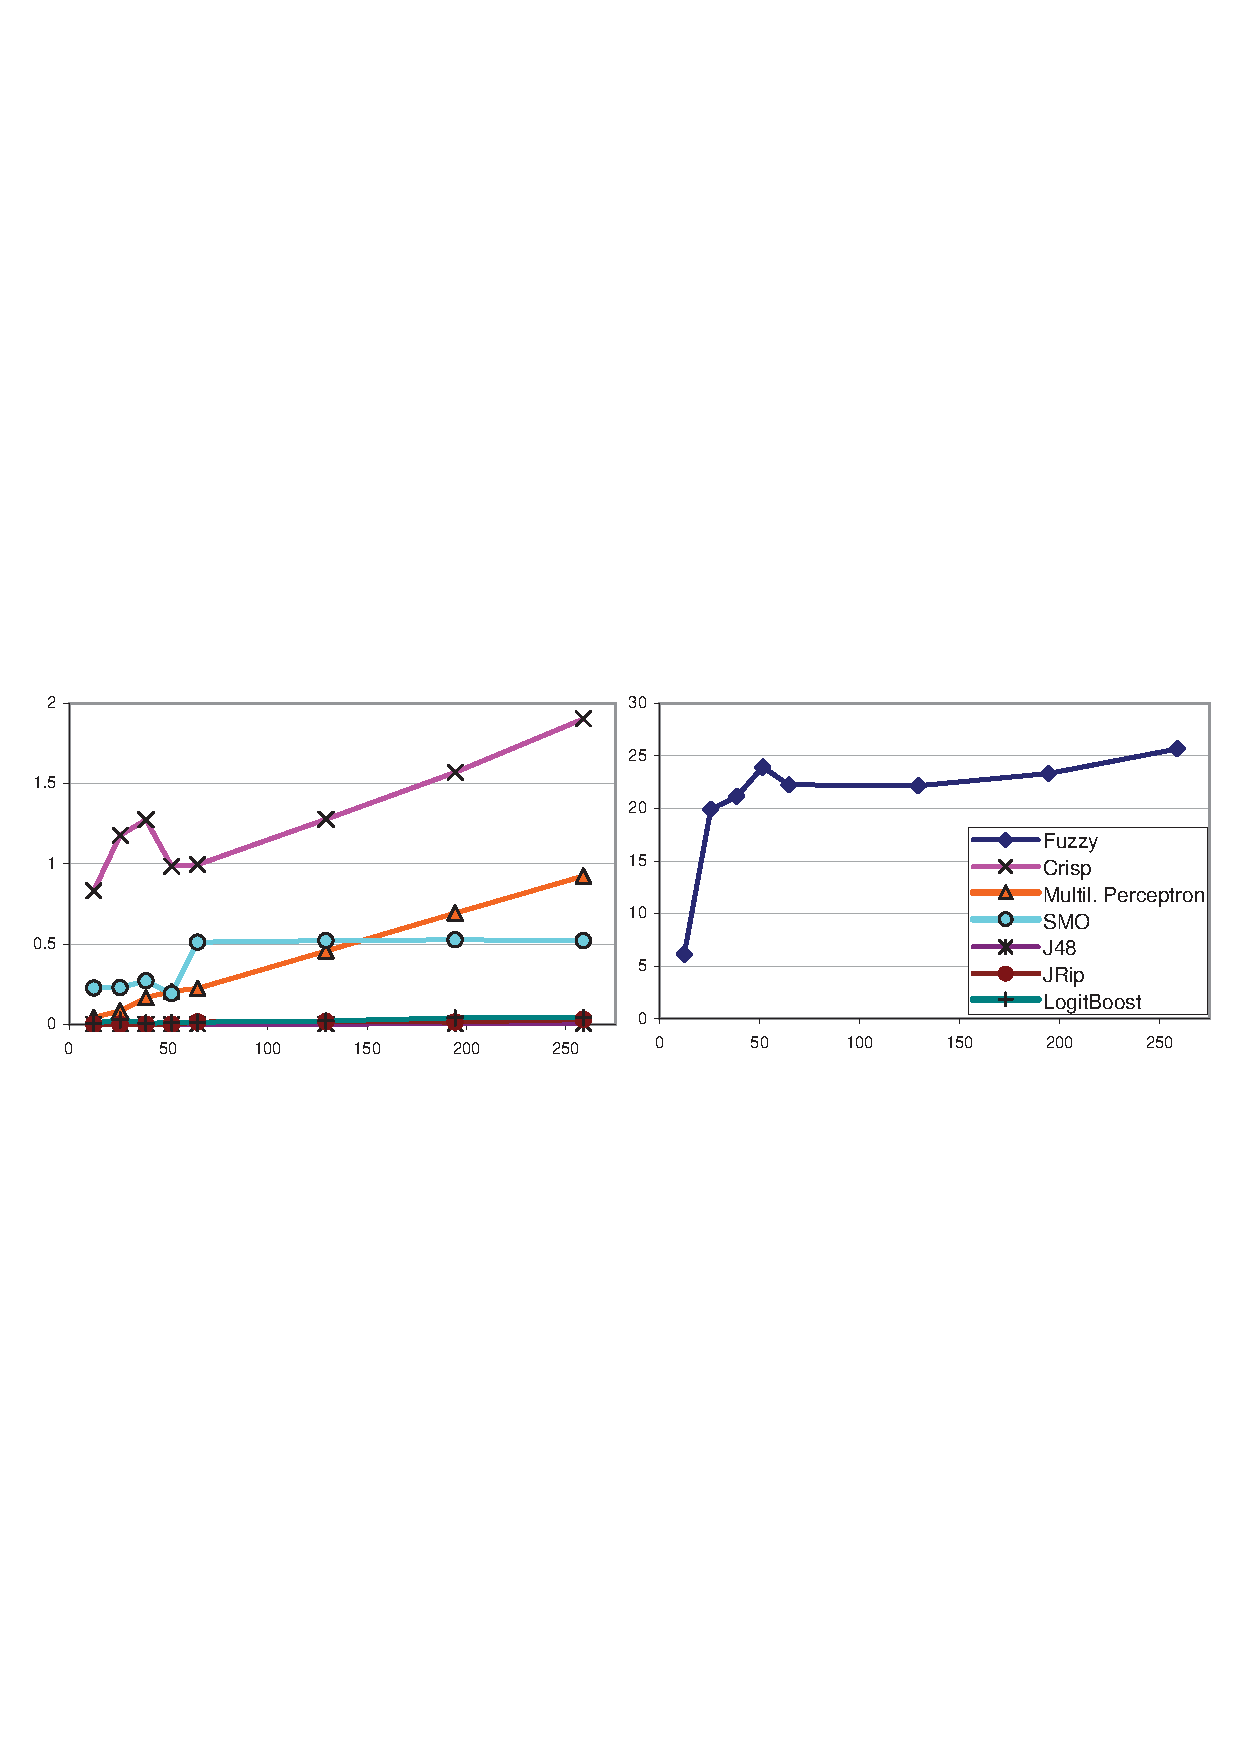
\includegraphics[width=\hsize]{learning_speed}}
\caption{x-axis: number of training instances, y-axis: training time in seconds, average values from 10 repetitions, `nursery' dataset.}
\label{img:learning_speed}
\end{figure}



%%%%%%%%%%%%%%%%%%%%%%%%%%%%%%%%%%%%%%%%%%%%%%%%%%%%%%%%%%%%%%%%%%%%%%%%%%%%%%%%%%%%%%%%%%%%%%%%%
\section{Conclusion} \label{sec:conclusion}
%%%%%%%%%%%%%%%%%%%%%%%%%%%%%%%%%%%%%%%%%%%%%%%%%%%%%%%%%%%%%%%%%%%%%%%%%%%%%%%%%%%%%%%%%%%%%%%%%
In this chapter we have presented a fuzzy system, which provides a fuzzy classification of textual web reports. Our approach is based on usage of third party linguistic analyzers, our previous work on web information extraction, and fuzzy inductive logic programming.

The main contributions are formal models, prototype implementation of the presented methods and an evaluation experiment. Our data and our implementation are publicly available on the Web. The first experiment evaluated performance of the presented methods and compared them with other machine learning procedures used in data mining on our data. The Fuzzy ILP classifier proved better results than a majority of the methods. The results are statistically significant in many cases. 
We see the advantage of the Fuzzy ILP classifier in the fact that monotonization leads to the extension of the learning domain and it utilizes the fact that the domain is or can be monotonically ordered.

In the second experiment, we evaluated all the methods on other datasets with more training instances and we also experimentally measured the time complexity of the methods. This experiment has shown that the fuzzy method is suitable mainly in situations with a small amount of training instances and in cases when the target attribute mostly respects the natural order of the remaining attributes. But this did not hold true for any of the later-used datasets. When comparing the fuzzy approach with the crisp one, the fuzzy approach always performed better in terms of correctness of the classification, but it was many times slower than all the methods in terms of time complexity.
